\section{Community} 
\label{sec:community}

As the purpose of preCICE is to connect different simulation software, preCICE naturally also helps connecting researchers -- imagine the fluid mechanics group and the solid mechanics group of a computational mechanics faculty with their individual in-house CFD and FEM codes.
In the last five years, a significant community of users has been formed around preCICE, with some of them also contributing back code or tutorials. The \textit{preDOM} project\footnote{More about preDOM on our blog: \url{https://precice.discourse.group/t/how-did-precice-get-popular/321}}, funded by the German Research Foundation, played an important role for this development. In fact, most of the improvements described in this paper were part of the project: building and packaging, adapters, tutorials, tests and continuous integration, but also user documentation and community building.   

Today, we know through forum discussions, conferences, workshops, and publications of more than 100 research groups using preCICE. Roughly one half of them are from academia, while the other half comes from non-academic research centers (e.g., the German Max Planck Institute for Plasma Physics, the German Helmholtz-Zentrum Hereon, the Italian Aerospace Research Centre, or A*STAR in Singapore) or industry (e.g., MTU Aero Engines or Bitron).   
We collect some user stories on our website\footnote{preCICE community stories: \url{https://precice.org/community-projects.html}}
and depict some highlights in \autoref{fig:testimonials}.
Presumably half of the users apply preCICE for fluid-structure interaction or conjugate heat transfer applications. The other half uses preCICE for more uncommon setups, for example, coupling of different fluid models with each other (e.g.,~\cite{revell2020coupled}) or coupling of CFD to particle methods (e.g.,~\cite{besseron2021eulerian}). 

\paragraph{Applications and Software}
A non-exhaustive list of application fields includes mechanical and civil engineering
(astronautics~\cite{Volland2019}, manufacturing processes~\cite{Seufert2019_COUPLED, scheiblhofer2019coupling}, aerodynamics~\cite{marinoinvestigation, folkersma2020steady, Cocco2020, Risseeuw2019, CINQUEGRANA2021103264, Huang2021_Helicopters, srivastava2019computational}, urban wind modeling~\cite{revell2020coupled}, aeroacoustics~\cite{Lindner2020_ExaFSA, kersschot2020simulation}, explosions~\cite{nguyen2015fluid, zhang2020numerical}), marine engineering~\cite{andrun2020simulating}, bio engineering (heart valves~\cite{Davis2019}, aortic blood flow~\cite{naseri2020scalable}, fish locomotion~\cite{luo2020fluid}, muscle-tendon systems~\cite{Maier2021_Diss}), nuclear fission and fusion reactors~\cite{deSantis2019, fan2020study, Desai2020_Fusion}, and geophysics~\cite{Jaust2020, schmidt2021simulation, geoKW}.
Many users do not only use the official adapters (cf.~\autoref{sec:adapters}), but couple further community codes or their in-house codes. A non-exhaustive list of available coupled software (under a commercial or an open-source license) includes CAMRAD II and TAU~\cite{Huang2021_Helicopters}, DUST~\cite{Cocco2020}, DuMuX~\cite{koch2021dumux, Jaust2020}, DUNE~\cite{Firmbach2021}, Rhoxyz~\cite{andrun2020simulating}, Ateles~\cite{klimach2014end}, XDEM~\cite{besseron2021eulerian}, and FLEXI~\cite{krais2021flexi}. 



\begin{figure}[h!]
\begin{minipage}{\textwidth}
\begin{minipage}{\dimexpr0.5\textwidth-10pt\relax}
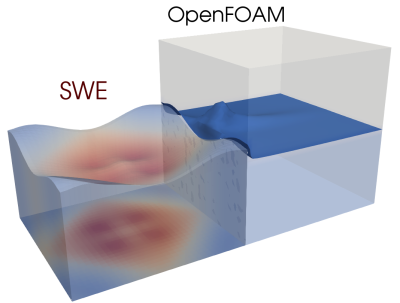
\includegraphics[width=\textwidth]{figs/testimonial-espinosa.png}
\end{minipage}\hfill
\begin{minipage}{\dimexpr0.5\textwidth-10pt\relax}
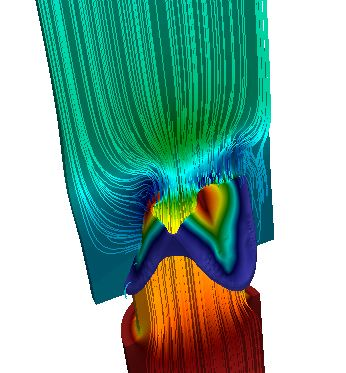
\includegraphics[width=0.8\textwidth]{figs/testimonial-south-africa.jpg}
\vspace{0.5cm}
\end{minipage}%
\end{minipage}
\begin{minipage}{\textwidth}
\begin{minipage}{\dimexpr0.45\textwidth-10pt\relax}
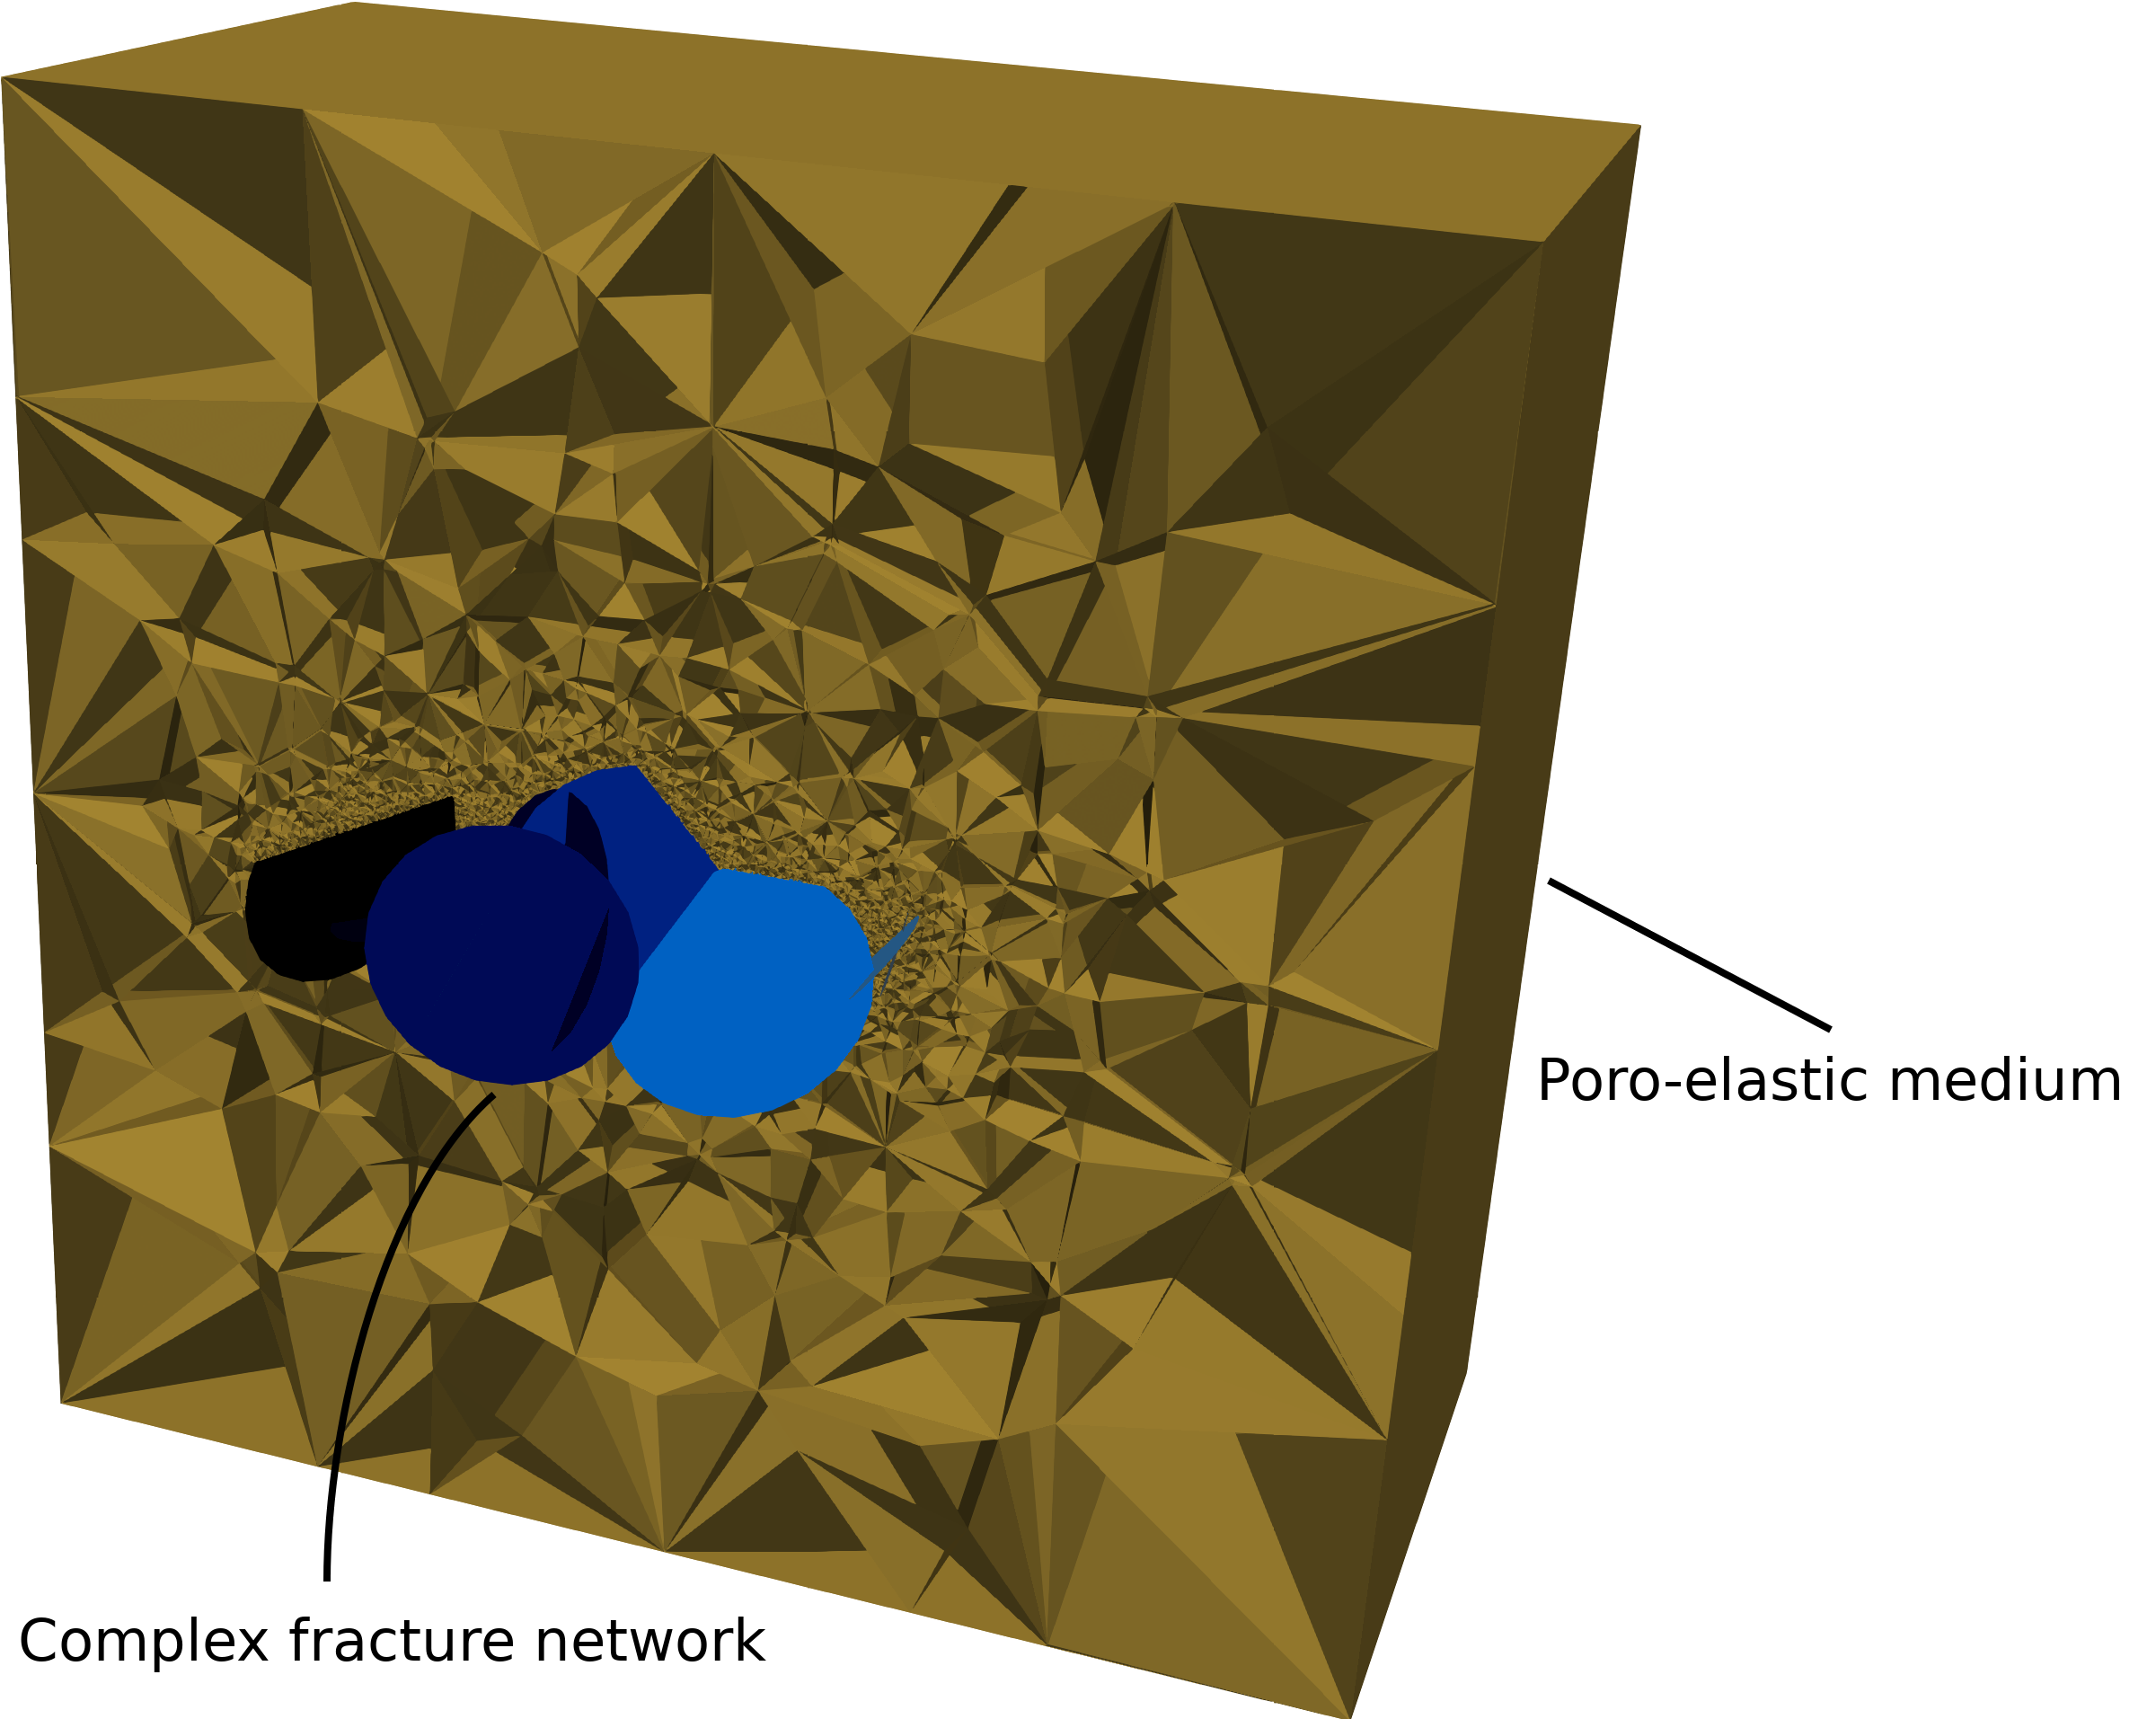
\includegraphics[width=\textwidth]{figs/testimonial-stuttgart-fractures.png}
\end{minipage}\hfill
\begin{minipage}{\dimexpr0.55\textwidth-10pt\relax}
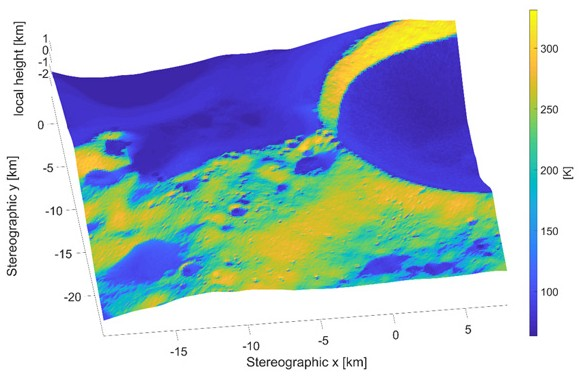
\includegraphics[width=\textwidth]{figs/testimonial-thermos.jpg}
\end{minipage}%
\end{minipage}
\caption{
\label{fig:testimonials}
Various simulations from the preCICE community. All pictures taken from the page \emph{Community stories} on \url{precice.org}. Top left: a shallow-water equations solver coupled to OpenFOAM~\cite{Espinosa2020}. Top right: an artificial heart valve simulated with OpenFOAM and CalculiX~\cite{Davis2019}. Bottom left: A 3D poro-mechanics model coupled to 2D fluid equations, both implemented in FEniCS~\cite{schmidt2021simulation}. Bottom right: a MATLAB heat equation solver coupled to a GPU ray-tracing software package to simulate heat conduction and radiation on the surface of the moon~\cite{Volland2019}.
}
\end{figure}

\paragraph{Community Building}
preCICE users can interact with developers and with each other through various channels. 
We provide and moderate a Discourse forum\footnote{preCICE forum on Discourse: \url{https://precice.discourse.group/}} and a Gitter chat room\footnote{preCICE chat room on Gitter: \url{https://gitter.im/precice/Lobby}}. 
The forum replaced a previously used mailing list as discussions in the forum can be much better structured through categories, labels, and \textit{solution} posts. Moreover, Discourse can be customized to great extent, which allows us to hand over moderation responsibilities to the community at a suitable pace.   
For feature requests and bug reports, we use the issue trackers of the different repositories on GitHub\footnote{preCICE GitHub organization: \url{https://github.com/precice}}. Moreover, we organize yearly mini-symposia at ECCOMAS conferences (ECCM-ECFD 2018, COUPLED 2019, WCCM 2020, COUPLED 2021) and our own preCICE Workshops (preCICE Workshop 2020 in Munich\footnote{Aftermath of the 2020 workshop: \url{https://precice.discourse.group/t/precice-workshop-2020-updates/40}}, preCICE Workshop 2021 online). The workshops include an introduction course, which we plan to further extend in the next years. \autoref{fig:traffic} shows a static growth of the preCICE community over the previous 3 to 4 years. 



\begin{figure}[h!]
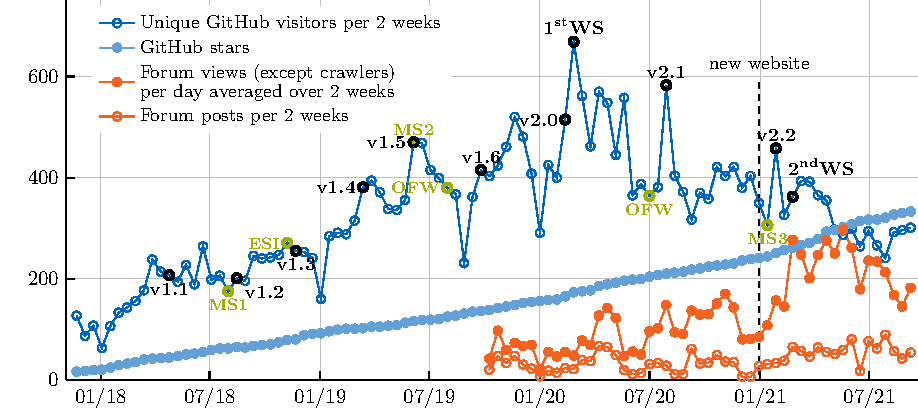
\includegraphics[width=0.95\textwidth]{figs/traffic/traffic.pdf}
\caption{
\label{fig:traffic}
Various traffic data showing community growth over time connected to key events. Whereas new releases have a clear impact on GitHub traffic, conferences, such as the ECCOMAS mini-symposia (MS1, MS2, MS3), different OpenFOAM workshops (ESI, OFW), and the preCICE workshops (WS) have not always a clear direct impact. With the start of the preCICE forum (fall 2019) and, in particular, with moving the user documentation to the new website at the end of 2020, traffic is shifted away from GitHub. At the online preCICE Workshop 2021, we used the forum to let attendees introduce themselves. This led to sustainable increase of forum traffic.
}
\end{figure}
  
  

\paragraph{Contributions}
To strengthen the sustainability of preCICE, we encourage users to also contribute back. Example contributions encompass code, tutorials, bug reports, or documentation. On our website, we provide detailed contributing guidelines\footnote{Contributing guidelines: \url{https://precice.org/community-contribute-to-precice.html}}. Our long-term goal is to hand over development of the official adapters (cf.~\autoref{sec:adapters}) to the community. In recent years, the OpenFOAM adapter has, in particular, seen various external contributions~\cite{nlrse19-chourdakis} and serves as an example of how the community may successfully contribute to isolated, smaller \emph{compartments} of a software project, as they can be easier to understand and contribute to. As of July 2021, 20\% (18 out of 89) pull requests and 26\% (26 out of 100) issues in the OpenFOAM adapter repository have been contributed by external contributors (not from the academic groups of the core team). While half of the external pull requests were ultimately not merged, they still serve as proof of concept for features that were at the time not aligned with the direction of the project. We have observed that several non-merged contributions were still useful for the community and we expect that tooling, automation, and clear guidelines will increase the ratio of successful external contributions in the long run.





 
 